\section{Serving in the Postconciliar Sanctuary}
Serving at Mass places you close to the holiest mysteries on earth. A good altar server knows not only the items carried in procession or handed to the priest, but also every vessel, book, and vestment around the sanctuary---including the consecrated vessels and clergy-reserved appointments that a server recognizes with reverence and never touches. Use Plate I to orient yourself across the sanctuary before checking each functional plate for exact handling boundaries, handoff cues, and immediate safety rules.

\PCDPlateHeader{Plate I --- The Postconciliar Roman Sanctuary}{Not to common scale (architectural perspective)}
\ifdefined\TriptychPrintEdition
\begin{center}
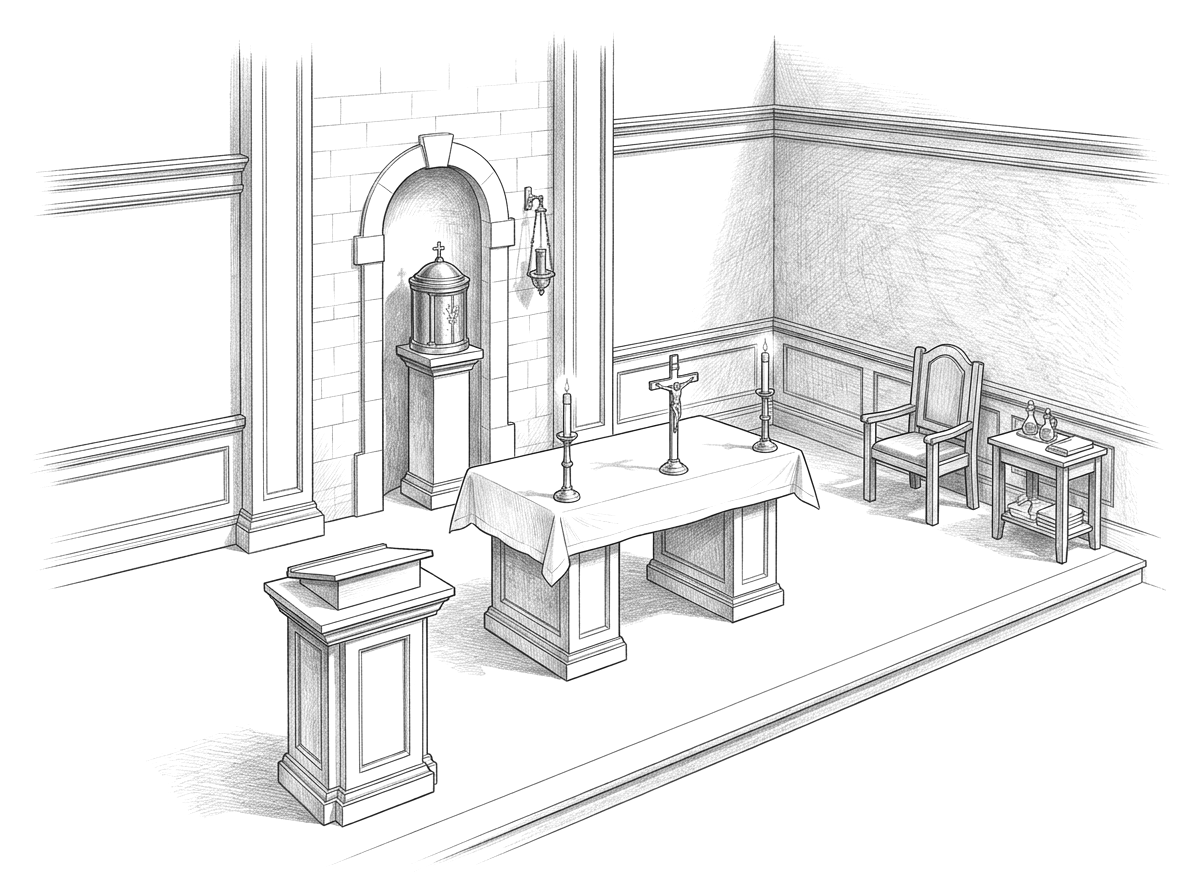
\includegraphics[width=0.96\linewidth,height=4.25in,keepaspectratio]{liturgy/roman-rite/postconciliar/2008-latin-2011-us-english/reference/roman-sanctuary-dictionary/shared/artwork/graphite/pc-art-01-sanctuary-composition.png}
\end{center}
\PCDPositionKey{Center: freestanding Altar with white Altar Cloth, two Altar Candles, and Altar Cross with corpus; foreground left: stationary Ambo; rear recessed niche: solid locked Tabernacle with hanging Sanctuary Lamp; rear right: Presidential Chair beside Credence Table holding cruets and linens.}
\else
\textbf{Visual Plate Summary (Plate I --- The Postconciliar Roman Sanctuary, Not to common scale (architectural perspective)):} Full architectural monochrome graphite perspective of a postconciliar Roman Catholic sanctuary showing the spatial coordination of freestanding stone altar dressed in white cloth with two candles and crucifix, permanent stone ambo in left foreground, wooden presidential chair and credence table with glass cruets and folded linens on the right, and a solid architectural tabernacle on a pillar inside a recessed arched niche with a hanging sanctuary lamp beside it. No altar cards, gradines, or rail appear.

\textbf{Reading order and object placement:} Center: freestanding Altar with white Altar Cloth, two Altar Candles, and Altar Cross with corpus; foreground left: stationary Ambo; rear recessed niche: solid locked Tabernacle with hanging Sanctuary Lamp; rear right: Presidential Chair beside Credence Table holding cruets and linens.
\fi

\subsection*{Knowing What You Handle and What Only Clergy Handle}
An altar server encounters many sacred things around the sanctuary, including vessels and books reserved strictly to the priest, deacon, or instituted acolyte. Each entry below marks whether you prepare, carry, or present the item, move it only when directed, or recognize it without touching it.
